\documentclass[journal]{IEEEtran}
\usepackage{amsmath,amsfonts}
\usepackage{algorithmic}
\usepackage{array}
\usepackage[caption=false,font=normalsize,labelfont=sf,textfont=sf]{subfig}
\usepackage{textcomp}
\usepackage{stfloats}
\usepackage{url}
\usepackage{verbatim}
\usepackage{graphicx}
\usepackage{multirow}
\usepackage{algorithm}
\usepackage{cite}
\usepackage{algorithmic}
\usepackage{array}
\usepackage{booktabs}
\usepackage{longtable}
\usepackage{multicol, lipsum}
\usepackage{tabularx}
\usepackage{svg}
\usepackage{booktabs} 
\usepackage[colorlinks,linkcolor=blue]{hyperref}
% left fixed width:
\newcolumntype{L}[1]{>{\raggedright\arraybackslash}p{#1}}

% center fixed width:
\newcolumntype{C}[1]{>{\centering\arraybackslash}p{#1}}

% flush right fixed width:
\newcolumntype{R}[1]{>{\raggedleft\arraybackslash}p{#1}}
\hyphenation{op-tical net-works semi-conduc-tor IEEE-Xplore}
\def\BibTeX{{\rm B\kern-.05em{\sc i\kern-.025em b}\kern-.08em
		T\kern-.1667em\lower.7ex\hbox{E}\kern-.125emX}}
\usepackage{balance}

\newcommand{\R}{\mathbb{R}}
\begin{document}
	\title{Probabilistic Refinement for RoI-based Monocular 3D Object Detection}
	\author{Tingyu Zhang, Zhigang Liang, Yanzhao Yang, Xinyu Yang, Yu Zhu, Jian Wang
		\thanks{Tingyu Zhang, Zhigang Liang, Yanzhao Yang, Yu Zhu and Jian Wang are with College of Computer Science and Technology, Jilin University, Changchun, China}
		\thanks{Xinyu Yang is with Automotive safety and Simulation Test Department, China Automotive Innovation Corporation, Nanjing, China}}
	
	\markboth{IEEE Transactions on Intelligent Vehicles}
	{Tingyu Zhang, Zhigang Liang, Yanzhao Yang, Xinyu Yang, Yu Zhu, Jian Wang:
		Contrastive Late Fusion for 3D Object Detection}
	
	\maketitle
	
	\begin{abstract}
	Monocular 3D object detection has garnered significant attention due to its cost-effectiveness and simplified setup. In this study, we delve into Region of Interest (RoI)-based monocular detectors. Previous approaches treat all parts of the RoI equally. However, different regions within the RoI hold varying importance, and accurate RoI estimation may be hindered by occlusions or long distances. Thus, we introduce the Multi-Scale Grid Attention (MSGA) mechanism to investigate multi-scale RoI exploration and the significance of RoI regions. Moreover, while existing methods treat depth estimation as a probability estimation during training, they do not effectively utilize probabilistic properties during inference. To tackle these issues, we propose a novel probabilistic post-processing method to enhance detection robustness. Experimental evaluations are conducted on the KITTI and Waymo datasets, achieving state-of-the-art performance.
	\end{abstract}
	
	\begin{IEEEkeywords}
		Camera, Intelligent vehicles, Monocular 3D object detection.
	\end{IEEEkeywords}
	

	\section{Introduction}
	\noindent\IEEEPARstart{M}{onocular} camera-based 3D object detection has become a significant research area in computer vision, with applications spanning autonomous driving, robotics, and augmented reality. Unlike conventional approaches dependent on depth sensors or multi-camera setups, monocular 3D object detection leverages the capabilities of a single camera to estimate the three-dimensional spatial information of objects within its field of view.
	
	The significance of monocular 3D object detection lies in its potential to provide depth perception using only the information captured by a single camera. This is particularly advantageous for real-world applications where cost, simplicity, and computational efficiency are essential considerations. Achieving accurate and robust 3D object detection from monocular images involves addressing complex challenges such as scale ambiguity, occlusions, and perspective distortions inherent to a single viewpoint.
	
	Monocular 3D object detection holds significance for its capability to infer depth using data from a single camera, offering advantages in real-world scenarios where cost, simplicity, and computational efficiency are critical. Ensuring accurate and reliable 3D object detection from monocular images requires tackling challenges including scale ambiguity, occlusions, and perspective distortions inherent to single viewpoints.
	
	The absence of explicit depth information poses a significant challenge for monocular 3D detectors, leading to a considerable disparity compared to point cloud-based methods. To bridge this gap, certain approaches~\cite{gupnet, didm3d, neurocs} initially forecast multiple Region of Interest (RoI) candidates and subsequently generate predictions for each. 3D RoI-based methods, such as those discussed in~\cite{neurocs}, often depend on pre-trained 3D monocular detectors. In contrast, 2D RoI-based methods solely predict 2D bounding boxes, offering a lighter and more efficient alternative. Furthermore, given the real-time demands of 3D object detection, efficiency is paramount. Therefore, this paper exclusively focuses on 2D RoI-based methods.
	
	2D Region of Interest (RoI)-based methods~\cite{gupnet, didm3d} typically involve three key steps. Firstly, the RoI is partitioned into distinct segments, followed by the application of RoI feature extraction techniques (such as RoI Pooling~\cite{fast-rcnn}, RoI Warp~\cite{roi-warp}, and RoI Align~\cite{mask-rcnn}) to extract pertinent features. Secondly, the RoI is fed into a neural network to further refine these features and generate predictions for each region. Finally, the individual predictions are integrated to yield the final results.
	
	\begin{figure}[!t]
		\centering
		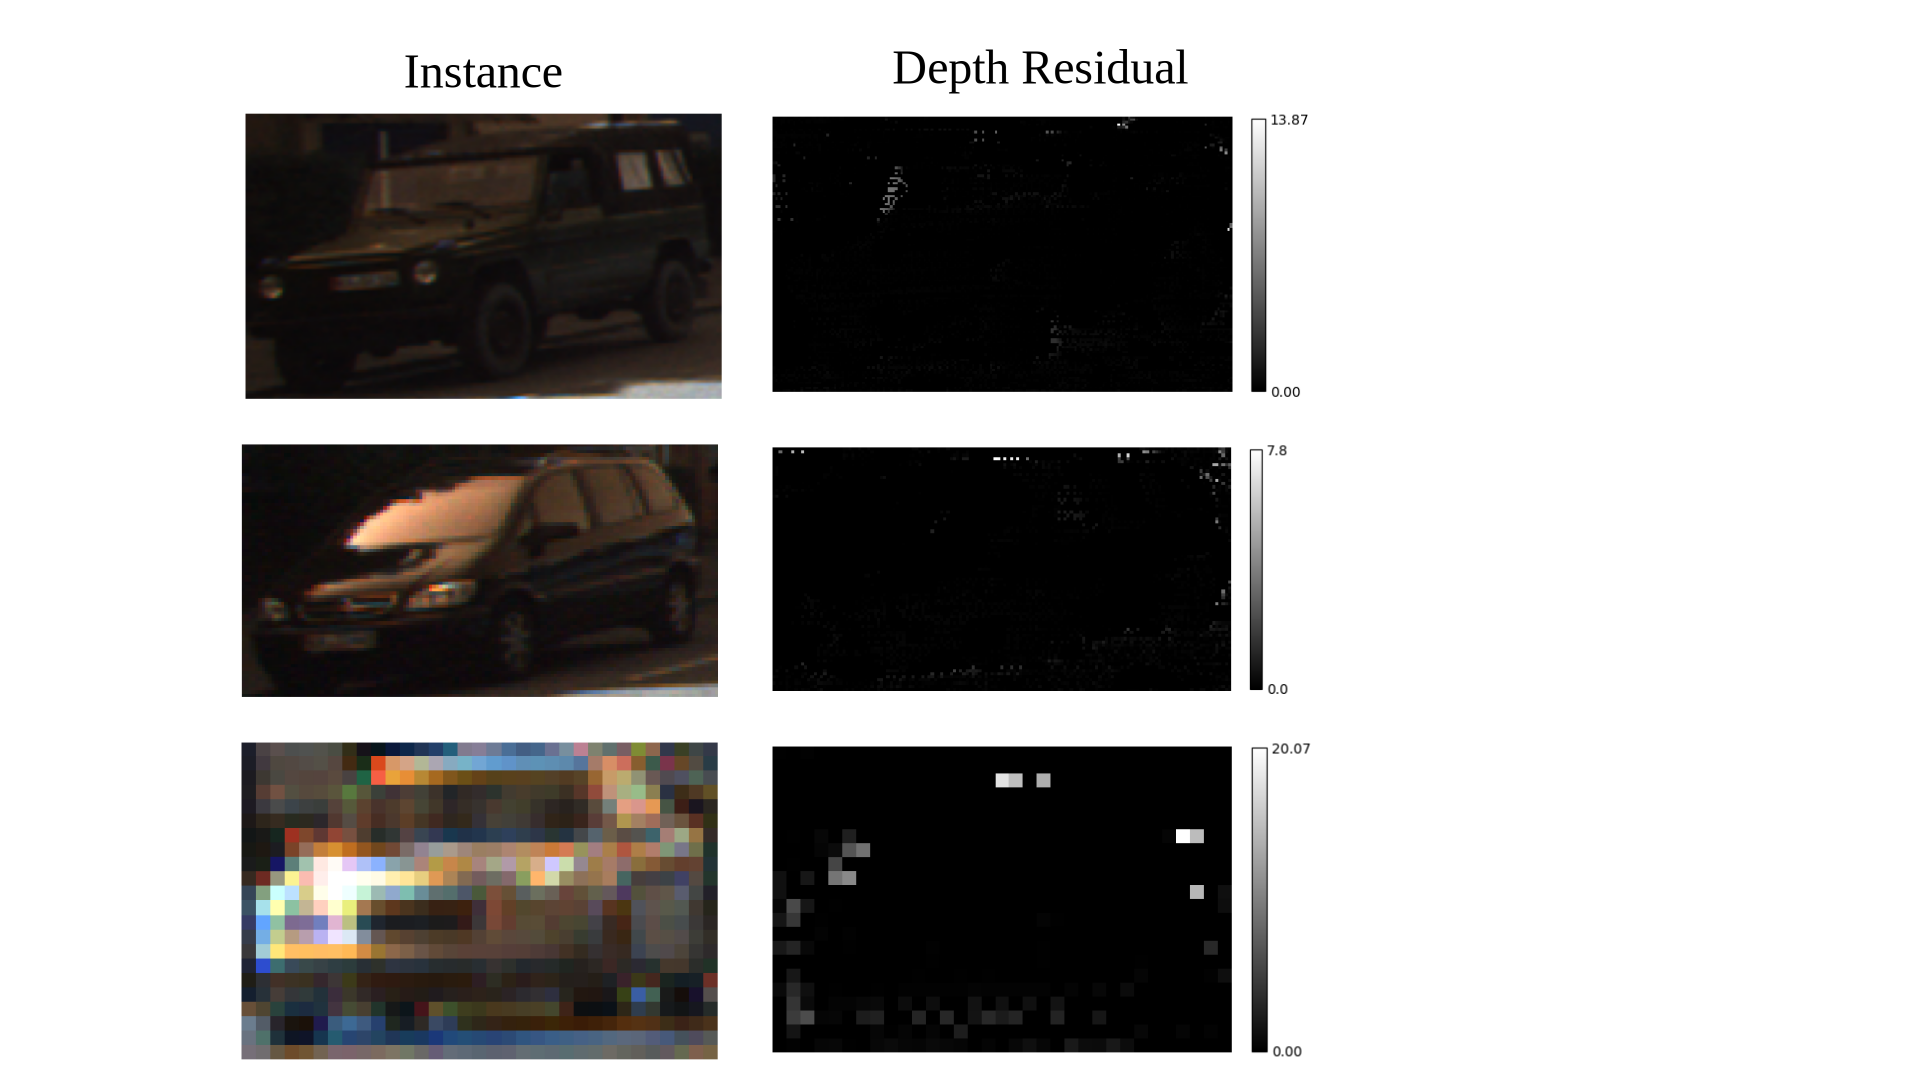
\includegraphics[width=1.0\linewidth]{Figures/depth_residual}
		\caption{Instance and Its Depth Residual. The depth residual of an instance is computed by taking the absolute difference between the predicted depth generated by the depth completion network and the corresponding ground truth. The left column shows the raw image of the instance, while the right column illustrates the depth residual. Lighter colors in the latter column indicate higher depth residuals.}
		\label{fig:depth_residual}
	\end{figure}

	However, the second and third steps present certain challenges. In the second step, each partition of the Region of Interest (RoI) is treated equally, disregarding the varying importance of different RoI regions. For instance, empirically, information pertaining to the tire or license plate number holds more significance than that concerning the car body, and background regions should have less influence than foreground areas. Taking DID-M3D~\cite{didm3d} as an example, it predicts the depth to the object surface, referred to as visual depth, to decouple the depth. In the KITTI~\cite{kitti} dataset, the training data for the depth completion task and 3D object detection task do not entirely overlap, resulting in some images in KITTI 3D lacking ground truth visual depth. Therefore, DID-M3D introduces a depth completion network to generate a dense visual depth map. We select images with labels and compare the ground truth with the depth map generated by the depth completion network. As depicted in Fig.~\ref{fig:depth_residual}, visual depth near the center of an object is more precise than at the edges. Taking the central visual depth of the RoI as the baseline, the distribution of visual depth in the RoI is unbalanced, as shown in Fig.~\ref{fig:visual_depth_offset}. Additionally, 2D RoIs are generated by the network, potentially resulting in incomplete object warping. To address these issues, we propose the Multi-Scale Grid Attention (MSGA) module. Specifically, we enlarge the RoI by adding various pixels to its size, extract multi-scale features using a network, and apply a Grid Attention (GA) module to assess the importance of different regions and further adjust the RoI features.

	\begin{figure}[!t]
		\centering
		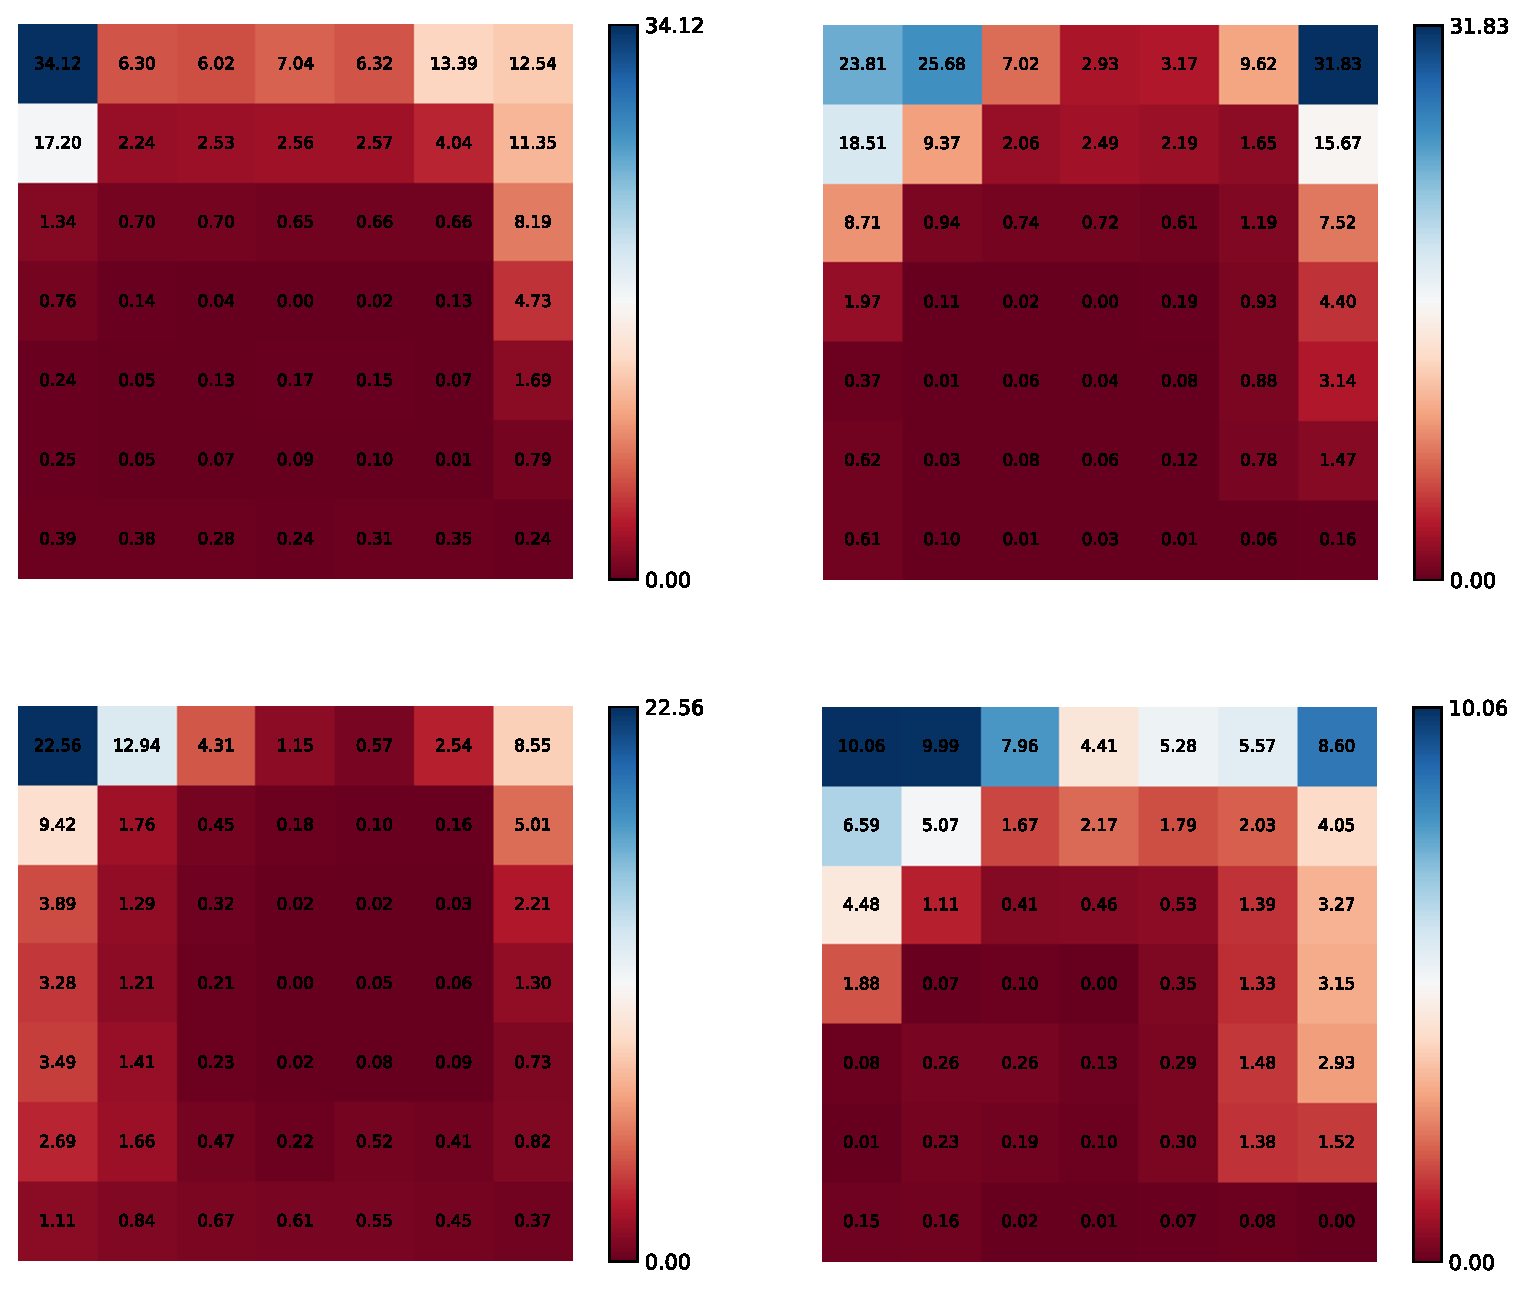
\includegraphics[width=1.0\linewidth]{Figures/visual_depth_offset/visual_depth_offset.eps}
		\caption{Visual Depth Offset: The visual depth of the central grid within the Region of Interest (RoI) is considered the baseline, from which the offset to other grids is computed. This absolute offset is subsequently labeled for each grid.}
		\label{fig:visual_depth_offset}
	\end{figure}
	
	In the third step, the results are integrated to obtain the final outcomes. Previous approaches commonly employed simple averaging or weighted summation. While adequate for properties like dimensions and position, where each grid shares the same regression target, this method encounters challenges in depth estimation. In particular, depth is decomposed into visual depth and attribute depth~\cite{didm3d}, as illustrated in Fig.~\ref{fig:decoupled_depth}. Each grid possesses distinct visual and attribute depths, leading to an imbalanced distribution that renders simple averaging suboptimal. Moreover, deriving the weights for weighted summation proves challenging. In our study, we adopt the assumption from previous research that depth follows a certain distribution, leveraging this probability distribution in the post-processing phase. This approach enhances the integration process's rationality.
	
	
	In summary, our contributions can be outlined as follows:
	\begin{itemize}
		\item We meticulously explore the limitations of 2D RoI-based monocular 3D object detection, highlighting an inconsistency in the significance of RoI grids. We introduce the notion of varying importance among RoI grids and propose the utilization of Multi-Scale Grid Attention to address this issue.
		\item During the post-processing phase, we meticulously consider the assumed depth distribution, employing probabilistic methods for refinement.
		\item The experimental results underscore the superiority of our method compared to existing approaches on the KITTI and Waymo datasets.
	\end{itemize}
	
	\section{Related Work}
	\subsection{Monocular 3D Object Detection without RoI}
	Given the inherent challenge of directly estimating instance depth with a monocular camera due to its ill-posed nature, previous studies have endeavored to leverage these constraints effectively. Mousavian et al. \cite{geometry3d} introduced constraints between 2D and 3D bounding boxes to formulate an equation group, integrating specific priors like driving direction to constrain the equation's degrees of freedom. PGD \cite{pgd} and MonoPair \cite{monopair} explore relationships between different instances, while DDMP-3D \cite{ddmp-3d} considers the relationships between neighboring pixels, utilizing these constraints to refine box estimations.
	
	Some alternative methods \cite{m3d-rpn, d4lcn, monodtr} employ numerous anchors placed on the 3D plane and extract anchor features through projection. These approaches encounter common issues associated with anchor-based methods, including the proliferation of anchors and the nontrivial configuration of anchor hyperparameters.
	
	Due to the scale variance in the image plane and the notable success of LiDAR detectors, several methods endeavor to convert the 2D image plane into the 3D plane. OFT \cite{oft} and ImVoxelNet \cite{imvoxelnet} utilize the projection of predefined 3D voxels onto the image plane to populate the features of each voxel. CaDDN \cite{caddn} partitions the depth range into segments and predicts the probability for each segment, followed by the expansion of pixel features into frustum features. MonoNeRD \cite{mononerd} leverages 2D image features to generate NeRF-like 3D representations. Additionally, various pseudo-LiDAR methods \cite{color-embeded, mono-plidar, patchnet} integrate an independent depth completion network to generate a dense depth map, using the calibration matrix to derive the pseudo LiDAR. Subsequently, a LiDAR-based detector is employed to obtain the final results. Despite its success, DD3D \cite{dd3d} argues that pseudo LiDAR is unnecessary for detection. Instead, it employs a single model to predict depth and 3D bounding box simultaneously, obviating the need for an independent depth completion network.
	
	Monocular 3D object detection heavily relies on accurate depth estimation~\cite{monodle}. Even slight errors in depth estimation can lead to objects being significantly offset from ground truth positions. To address this challenge, many methods aim to introduce additional supervision to constrain depth offsets. Key point estimation, as demonstrated in works such as Polygon~\cite{polygon}, is commonly employed because it imposes eight additional constraints on the model. Representative methods utilizing this approach include RTM3D~\cite{rtm3d}, SMOKE~\cite{smoke}, MonoDDE~\cite{monodde}, and Monocon~\cite{monocon}.
	
	There are several methods that employ other different strategies to improve performance. For instance, M3DSSD~\cite{m3dssd}, MonoPGC~\cite{monopgc}, CIE~\cite{cie}, and SSD-MonoDETR~\cite{ssd-monodetr} incorporate attention mechanisms to enhance performance. MonoFlex~\cite{monoflex} specifically addresses truncated objects by predicting edge heatmaps for them.
	
	\subsection{Monocular 3D Object Detection with RoI}
	
	RoI-based object detection can be broadly categorized into 3D RoI-based and 2D RoI-based methods. 3D RoI-based approaches~\cite{neurocs, monoxiver} typically depend on a separately pretrained monocular 3D object detector to produce 3D proposals, a process that may not meet the real-time demands of autonomous driving. In contrast, 2D RoI-based methods~\cite{roi10d, didm3d, gupnet, gupnet++} share most of the network in both RoI generation and object detection, rendering them more efficient.
	
	In this study, our emphasis is on 2D RoI-based methods. Recognizing the challenges posed by RoI generation noise and the varying significance of RoI components, we introduce the Multi-Scale Grid Attention (MSGA) module to effectively address these issues. Additionally, we introduce a novel probabilistic post-processing strategy to leverage the probabilistic assumptions inherent in depth estimation.
	\begin{figure*}[!t]
	\centering
	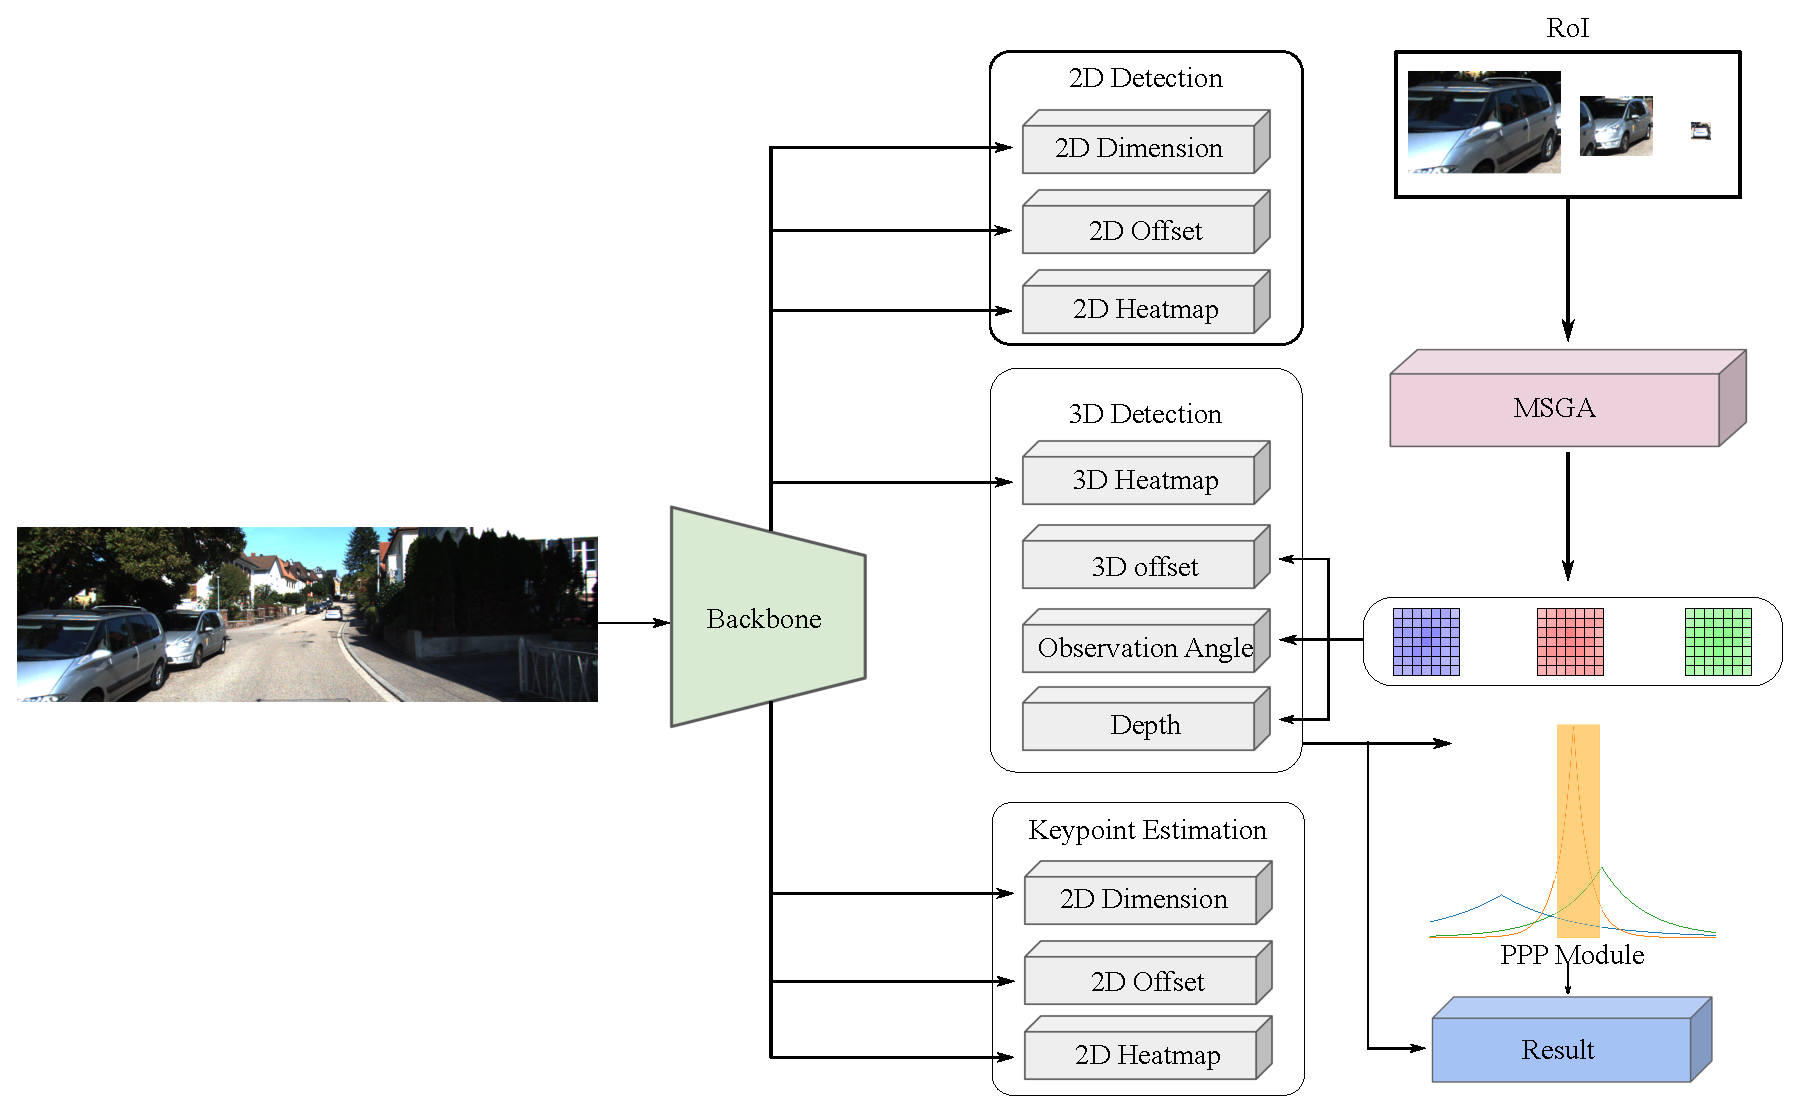
\includegraphics[width=1.0\linewidth]{Figures/overview/overview.eps}
	\caption{Overview of our model. Initially, the input image undergoes processing through the backbone network to extract image features. These features are subsequently utilized for 2D detection, keypoint estimation, and 3D heatmap generation. Leveraging the results of 2D detection, the Region of Interest (RoI) features are directed to the Multi-Scale Grid Attention (MSGA) module for refinement. The enhanced RoI features are then employed to predict the 3D offset, observation angle, and depth. The depth estimation undergoes optimization via the Probabilistic Post-Processing (PPP) module. Finally, the results are decoded by both 3D properties and optimized depth.}
	\label{fig:overview}
\end{figure*}
	
	\section{Method}\label{sec:method}
	\subsection{Problem Definition}
	In the domain of monocular 3D object detection, the primary input consists of the RGB image $I$. The main goal is to determine essential properties of the 3D bounding boxes, including the 3D center coordinates $x_c, y_c, z_c$, the 3D dimensions $l, w, h$ and the observation angle $\theta$, which is more related to image appearance than orientation angle~\cite{geometry3d}. A crucial element in this procedure is the projection matrix $P$, as described in Eq.~\eqref{eq:projection_matrix}.
	\begin{equation}
		P=\begin{pmatrix}f&0&c_u&-fb_x\\0&f&c_v&-fb_y\\0&0&1&-fb_z\end{pmatrix}
		\label{eq:projection_matrix}
	\end{equation}

	where $f$ denotes the focal length, while $c_u$ and $c_v$ denote the vertical and horizontal positions of the camera in the image, respectively. Furthermore, $b_x$, $b_y$ and $b_z$ indicate the baseline relative to the reference camera. Notably, these values are non-zero in the KITTI dataset and zero in the Waymo dataset.
	
	In a monocular setting, determining the 3D center position poses a significant challenge, mainly due to the considerable variability in 3D center scale. As a result, many studies opt to predict the projected 3D center on the image plane, denoted as $x_{ic}, y_{ic}$, along with the corresponding depth $d$.The recovery of the 3D bounding box center is then accomplished using Eq.~\eqref{eq:projection}.
	\begin{equation}
		dx_{2d} = Px_{3d}
		\label{eq:projection}
	\end{equation}

	where $P$ denotes the projection matrix, $x_{3d}$ represents the 3D bounding box center $(x_c, y_c, z_c, 1)^T$, $x_{2d}$ signifies the projected 3D center on the image plane $(x_{ic}, y_{ic}, 1)^T$, and $d$ denotes the depth of $x_{3d}$.
	
	\subsection{Overview}
	The schematic overview of our methodology is depicted in Figure~\ref{fig:overview}. Initially, the provided image $I$ is processed through the image backbone, as discussed in Section~\ref{backbone}. Subsequently, a 2D detection head is employed to extract 2D properties, including the width and height of the bounding box, and to generate the heatmap for the projected 3D object center, as elaborated in Section~\ref{2d_detection_head}. Key point estimation, following the methodology of Monocon~\cite{monocon}, is incorporated into our approach. Utilizing the heatmap in conjunction with the predicted width and height, the 2D Region of Interest (RoI) is determined. The RoI is then input into the Multi-Scale Grid Attention (MSGA) module to refine the features, as explained in Section~\ref{msga}. Employing the DID-M3D~\cite{didm3d} approach for each RoI grid, we predict both the visual depth and attribute depth, enabling subsequent prediction of 3D properties such as dimensions and observation angle. In the post-processing phase, we apply a novel depth integration strategy to consolidate RoI depths, taking into account the practical significance of probability distribution. This strategy is outlined in Section~\ref{post_processing}..
	
	\subsubsection{Image Backbone}\label{backbone}
	Given an input RGB image $I$ with dimensions $3 \times H \times W$, we utilize a feature backbone $f(\cdot; \Theta)$ to compute the feature map $F$ with dimensions $D \times h \times w$:
	\begin{equation}
		F = f(I;\Theta)
		\label{eq:backbone}
	\end{equation}

	where $\Theta$ represents all learnable parameters, $D$ denotes the output feature map dimension (e.g., $D=512$), and $h$ and $w$ are determined by the overall subsampling rate $s$ in the backbone (e.g., $s=4$). To ensure fair comparisons in our experiments, we employ the DLA-34~\cite{dla} network as our chosen backbone.
	
	\subsubsection{2D Detection Head}\label{2d_detection_head}
	Utilizing the output feature map $F$ from the backbone as input, we route it through three detection heads. Each detection head comprises a series of operations: a 2D convolution, Rectified Linear Unit (ReLU) activation function, followed by another 2D convolution. Specifically, the first detection head is responsible for predicting the heatmap $H$ indicating the projected 3D object center. The process of heatmap generation follows the methodology outlined in CenterNet~\cite{centernet}. The second detection head focuses on predicting the offsets $\Delta x$ and $\Delta y$ between the projected 3D object center and the center of the 2D bounding box. Finally, the third detection head is tasked with predicting the width $w_{2d}$ and height $h_{2d}$ of the 2D bounding box.
	
	\subsubsection{Multi-Scale Grid Attention Module}\label{msga}
	During the training phase, we utilize the ground truth projected 3D object center $(x_{c_{gt}}, y_{c_{gt}})$, predicted offsets $\Delta x$ and $\Delta y$, as well as the predicted width $w_{2d}$ and height $h_{2d}$ of the 2D bounding box to compute the Region of Interest (RoI) using Eq~\eqref{eq:RoI_generation}.	
	\begin{equation}
	\begin{aligned}
	RoI =& (x_{c_{gt}}-w_{2d}/2, y_{c_{gt}}-h_{2d}/2, \\
  &x_{c_{gt}}+w_{2d}/2, y_{c_{gt}}+h_{2d}/2)
	\label{eq:RoI_generation}
	\end{aligned}
	\end{equation}
	During the inference phase, we select the top 50 positions from the heatmap to represent the predicted projected 3D object center. Subsequently, we combine the predicted offset and 2D dimensions to generate the RoI.

	Adjacent background pixels are crucial for discriminating foreground pixels. In point cloud-based 3D object detection, such as in Pyramid-RCNN, 3D Regions of Interest (RoI) also encounter similar challenges. Enlarging the RoI is a common strategy to mitigate this issue. In Pyramid RCNN~\cite{pyramid-rcnn}, the RoI is expanded proportionally based on the original RoI, as in 3D dimensions, the scale remains constant, implying that objects maintain the same dimensions regardless of distance. However, in the image plane, the scale varies with distance. Proportional enlargement may not be optimal, potentially introducing excessive background pixels for nearby objects. Thus, we enlarge the RoI by a fixed number of pixels. Determining the required pixels for RoIs with different sizes and varying accuracies of 2D bounding box prediction is challenging. To address this, we propose a Multi-Scale configuration, depicted in Fig~\ref{fig:multi-scale-grid-attention}. The original RoI is cropped by the predicted 2D bounding box. We uniformly increase the width and height of the 2D bounding box by 10 and 20 pixels, respectively, to create the enlarged RoI. Subsequently, RoI Align~\cite{mask-rcnn} is applied to generate $7\times 7$ RoI features. A $1\times 1$ convolution generates the attention map for each grid. The RoI feature is then multiplied by the attention map, and the result is added to the RoI feature to obtain the merged feature. Finally, the multi-scale merged features are concatenated to form the final feature.

The Multi-Scale Grid Attention (MSGA) module comprises two components: the multi-scale Region of Interest (RoI) feature and the Grid Attention mechanism. The benefits of the multi-scale RoI feature are outlined below:
\begin{itemize}
	\item Enhanced Inclusion of Foreground Pixels: Multi-scale features mitigate errors in 2D bounding box predictions, improving the likelihood of encompassing foreground pixels.
	\item Improved Background Information Utilization: By incorporating adjacent background pixels, multi-scale features enable better extraction of information from the background region.
\end{itemize}

The advantages of the Grid Attention mechanism are summarized as follows:
\begin{itemize}
	\item Discriminative Pixel Attention: While adjacent background pixels aid in model training, their importance is inferior to that of foreground pixels. Grid Attention facilitates the discrimination between background and foreground pixels.
	\item Importance Discrimination Among Foreground Pixels: Notably, within foreground pixels, certain elements hold greater significance. For example, a license plate serves as an iconic identifier for a vehicle.
\end{itemize}

	
	
	
	
	\begin{figure}[!t]
		\centering
		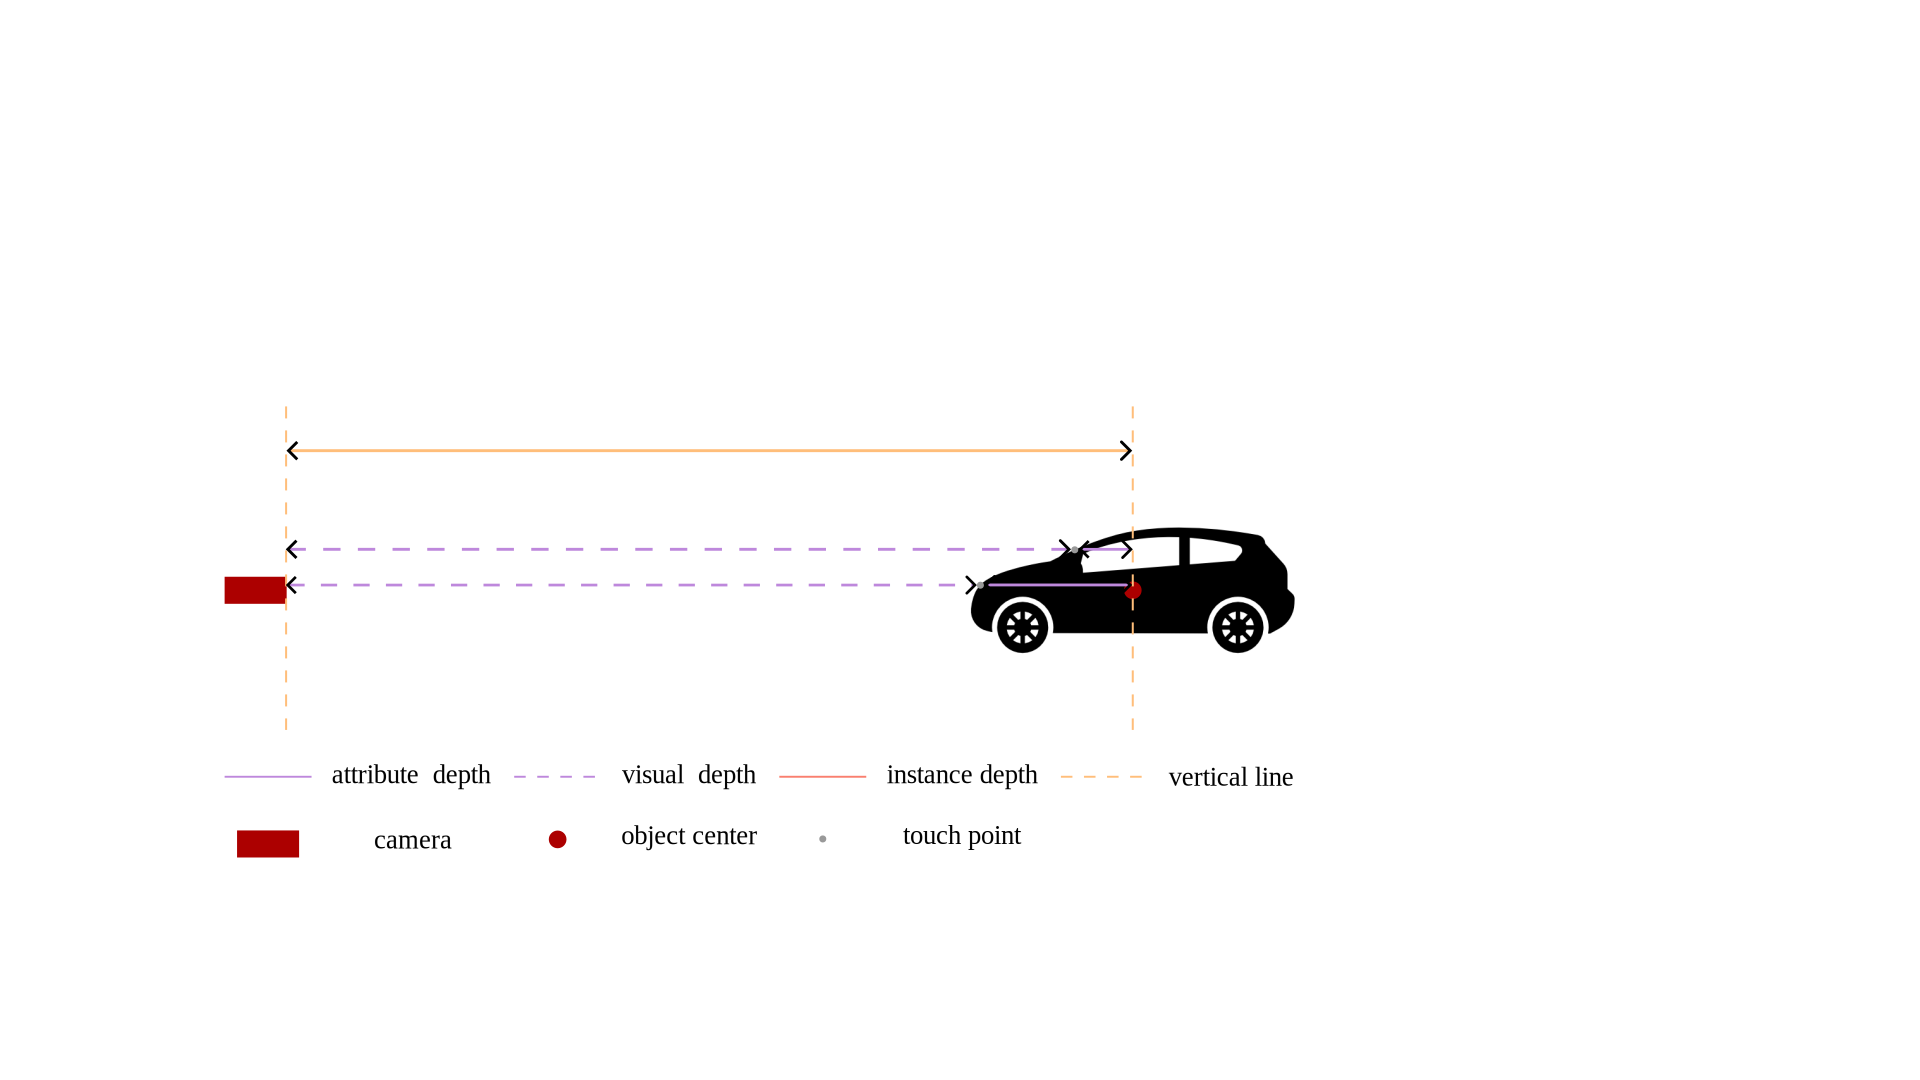
\includegraphics[width=1.0\linewidth]{Figures/decoupled_depth_fig/decoupled_depth.eps}
		\caption{Decoupled depth. The instance depth is defined as the distance between the object center to the camera plane. And the visual depth is distance of object surface to the camera plane. The attribute depth is obtained by the minus of instance depth and visual depth.}
		\label{fig:decoupled depth}
	\end{figure}
	
	\subsubsection{3D Detection Head}\label{3d_detection_head}
	
	For each set of RoI features, we employ seven distinct detection heads to predict various properties. These include the 3D dimensions offset, denoted as $dim_{3d}$, in comparison to the mean size of each class; the offset $offset_{3d}$ representing the quantization error-induced displacement between the projected 3D object center and the corresponding pixel; the visual depth $d_{vis}$ and its associated uncertainty $\sigma_{vis}$; the attribute depth $d_{att}$ and its corresponding uncertainty $\sigma_{att}$; and the observation angle $\theta$. The description of visual depth, attribute depth and instance depth is illustrated in Fig.~\ref{fig:decoupled depth}. 
	
	The detection heads responsible for predicting $dim_{3d}$, $offset_{3d}$, and $\theta$ consist of a sequence comprising a 2D convolution layer followed by Batch Normalization, Rectified Linear Unit (ReLU), and another 2D convolution layer. Conversely, the detection heads tasked with predicting $d_{vis}$, $\sigma_{vis}$, $d_{att}$, and $\sigma_{att}$ are composed of a 2D convolution layer, LeakyReLU activation function~\cite{leaky-relu}, and another 2D convolution layer.
	
	\subsubsection{Loss Functions}
	\paragraph{2D Heatmap} The 2D detection head generates three outputs: the heatmap $H$, the offset $\Delta x, \Delta y$, and the 2D dimensions $(w_{2d}, h_{2d})$. Our loss function follows the methodology outlined in CenterNet~\cite{centernet}. To guarantee a bounding box overlap of at least 0.7 IoU with the ground truth, we calculate the radius accordingly. Specifically for $H$, we utilize a modified focal loss, defined as follows:
	
	\begin{equation}
		\begin{split}
		L_{heat}=\frac{-1}N\sum_{H}\begin{cases}(1-H)^\alpha\log(H)&\text{if }\hat{H}=1\\(1-\hat{H})^\beta({H})^\alpha \\ \log(1-{H}) &\text{otherwise}\end{cases}
		\label{eq:heatmap loss}
		\end{split}
	\end{equation}

	where $\hat{H}$ denotes the target heatmap, with $N$ representing the number of keypoints in the image. For our experiments, we set the hyper-parameters $\alpha$ and $\beta$ for the focal loss to 2 and 4, respectively.
	
	\paragraph{2D Box} 
	For the 2D bounding boxes, we predict the offsets between the peak in the 2D heatmap $H$ and the center of the 2D bounding box, denoted as $\Delta x_{2d}$ and $\Delta y_{2d}$, along with the sizes of the bounding box, represented by $h_{2d}$ and $w_{2d}$. These values are determined using the L1 loss, as formulated in Eq~\eqref{eq:2d box loss}.
	\begin{equation}
		L_{box_{2d}} = \sum_{o\in \{\Delta x_{2d}, \Delta y_{2d}, w_{2d}, h_{2d}\}}\lvert o - \hat{o} \rvert
		\label{eq:2d box loss}
	\end{equation}
	where $o$ denotes the predicted value and $\hat{o}$ denotes the regression target.
	\paragraph{3D Box}
	For 3D box, we need to regress the offset between the peak in 2D heatmap and the projected 3D object center $\Delta x_{3d}, \Delta y_{3d}$, along with the offset of ground truth dimensions and the averaged dimensions $\Delta l_{3d}, \Delta w_{3d}, \Delta h_{3d}$. They are all calculated by the L1 loss, which is formulated as Eq~\eqref{eq:3d box loss}.
	\begin{equation} 
		L_{box_{3d}} = \sum_{o\in \{\Delta{x_{3d}}, \Delta{y_{3d}}, \Delta l_{3d}, \Delta w_{3d}, \Delta h_{3d}\}}\lvert o - \hat{o} \rvert
		\label{eq:3d box loss}
	\end{equation}

	\paragraph{Depth}
	To predict the 3D bounding box, we must regress the offsets between the peak in the 2D heatmap and the projected 3D object center, denoted as $\Delta x_{3d}$ and $\Delta y_{3d}$, as well as the offsets between the ground truth dimensions and the averaged dimensions, represented by $\Delta l_{3d}$, $\Delta w_{3d}$, and $\Delta h_{3d}$. These values are calculated using the L1 loss, as formulated in Eq~\eqref{eq:3d box loss}.
	\begin{equation} 
		L_{depth} = \sum_{*\in \{vis, att, ins\}} \frac{\sqrt{2}}{e^{\frac{u_*}{2}}} \times \lvert d_* - \hat{d_*} \rvert + \frac{u_*}{2}
		\label{eq:depth loss}
	\end{equation}

	where $d_{vis}$, $d_{att}$, and $d_{ins}$ represent the visual depth, attribute depth, and instance depth, respectively, while $u_{vis}$, $u_{att}$, and $u_{ins}$ denote the uncertainty associated with each depth. The symbol $\hat{d_*}$ denotes the regression target. It is important to emphasize that our network predicts only the visual depth and attribute depth, with the instance depth calculated as the sum of these two. Furthermore, the uncertainty is trained using non-supervised methods.
	
	\paragraph{Orientation Angle}
	We employ the Multi-bin loss for the orientation angle. Specifically, we partition $2 \pi$ into 12 bins, and the network generates the classification vector $\theta_{cls}$ to identify the bin in which the angle lies, along with the offset $\theta_{reg}$ between the bin center and the ground truth angle. The cross-entropy loss is utilized for $\theta_{cls}$, as formulated in Eq~\eqref{eq:angle loss}.
	\begin{equation} 
		L_{angle_{cls}} = -\sum_{i=1}^{12} y_{i}\log(p_{i})
		\label{eq:angle loss}
	\end{equation}

	where $y_i$ as the indicator for the $i$th bin, where it equals 1 if the angle falls within the bin, and 0 otherwise. $p_i$ represents the predicted probability of the $i$th bin. As for $\theta_{reg}$, we employ the L1 loss, as formulated in Eq~\eqref{eq:angle reg loss}.
	
	
	\begin{equation} 
		L_{angle_{reg}} = \lvert \theta_{reg} - \hat{\theta_{reg}} \rvert
		\label{eq:angle reg loss}
	\end{equation}

	where $\hat{\theta_{reg}}$ is the regression target.
	
	\paragraph{Keypoints}
	We incorporate an auxiliary keypoint loss inspired by Monocon~\cite{monocon}. To generate the keypoint heatmap $H_k \in \R^{9 \times w \times h}$, we project the eight corners and the 3D object center onto the image plane, thus representing nine keypoints. The loss function mirrors that of the 2D heatmap, albeit with a stricter IoU threshold of 0.3, as adopted in Monocon~\cite{monocon}. This loss function is detailed in Eq~\eqref{eq:keypoint heatmap loss}.
	\begin{equation}
	\begin{split}
		L_{H_k}=\frac{-1}N\sum_{H_k}\begin{cases}(1-H_k)^\alpha\log(H_k)&\text{if }\hat{H_k}=1\\(1-\hat{H_k})^\beta({H_k})^\alpha \\ \log(1-{H_k}) &\text{otherwise}\end{cases}
		\label{eq:keypoint heatmap loss}
	\end{split}
	\end{equation}
	
	In addition to the keypoint heatmap, we also predict the offset between each keypoint and the projected 3D object center pixel, denoted as $\Delta k2c_x$ and $\Delta k2c_y$, along with the offset between the peak in the keypoint heatmap and the keypoint position, represented as $\Delta kx$ and $\Delta ky$. These offsets are all calculated using the L1 loss, as formulated in Eq.~\eqref{eq:keypoint loss}.
	\begin{equation}
		L_{keypoint} = \sum_{i=1}^{12}\sum_{o\in \{\Delta k2c_x, \Delta k2c_y, \Delta kx, \Delta ky\}}\lvert o^i - \hat{o^i} \rvert
		\label{eq:keypoint loss}
	\end{equation}
	
	where $o^i$ denotes the prediction of the $i$-th keypoint, while $\hat{o^i}$ signifies the target corresponding to the $i$-th keypoint.
	
	The total loss is computed as the summation of the aforementioned losses, as defined in Eq. \eqref{eq:total loss}.
	\begin{equation}
	\begin{aligned}
		L_{total} =& L_{heat} + L_{box_{2d}} + L_{box_{3d}} + L_{depth} +\\ 
		& L_{angle_{cls}} + L_{angle_{reg}} + L_{H_k} + L_{keypoint}
		\label{eq:total loss}
	\end{aligned}
	\end{equation}
	\begin{figure*}
		\centering
		\includegraphics[width=1.0\linewidth]{Figures/multi-scale/Multi-Scale-Grid-Attention.eps}
		\caption{Multi-Scale Grid Attention Module. We use three scale to generate the RoI, the RoI feature is obtained by RoI Align. We use 1D convolutional network to generate the attention map of RoI grid. Then we multiply the attention map and the RoI feature, fed to residual summation for the merged feature. The final feature is integrated by the multi-scale merged feature.} 
		\label{fig:multi-scale-grid-attention}
	\end{figure*}
	
	\begin{figure}[!t]
		\centering
		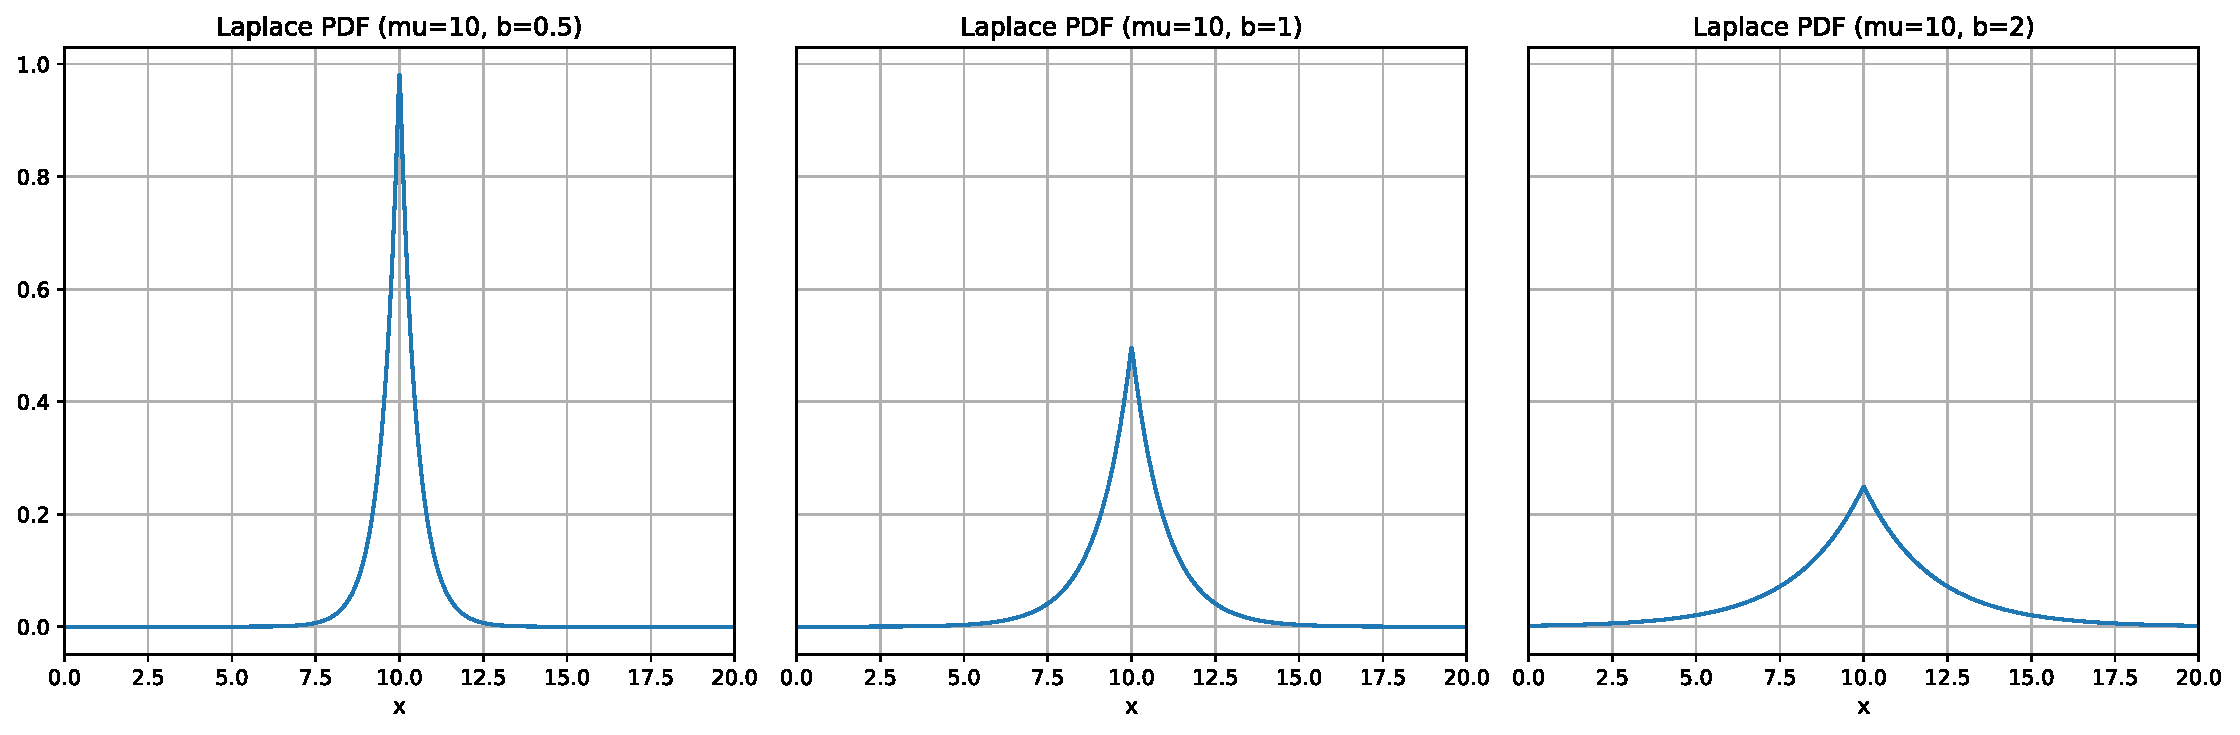
\includegraphics[width=1.0\linewidth]{Figures/laplace/laplace_distribution}
		\caption{Laplace Probability Density Function. Left distribution means $\mu=10, b=0.5$. Middle distribution means $\mu=10, b=1$. Right distribution means $\mu=10, b=2$.}
		\label{fig:laplace distribution}
	\end{figure}
	\subsection{Probabilistic Post Processing}\label{post_processing}
		Previous studies have assumed that depth adheres to the Laplace distribution. The Probability Density Function (PDF) of the Laplace distribution is defined as shown in Eq. \eqref{eq:laplace pdf}. 
		\begin{equation}
			f(x|\mu,b)=\frac1{2b}\exp\left(-\frac{|x-\mu|}b\right)
			\label{eq:laplace pdf}
		\end{equation}
		
		Fig. \ref{fig:laplace distribution} illustrates that as $b$ decreases, the curve becomes flatter, while increasing $b$ results in a more pointed curve.
		
		Previous methods have utilized the standard deviation $\sigma$ to assess the accuracy of depth estimation, employing $e^{-\sigma}$ to gauge the confidence level of the estimation. However, the rationale behind importance estimation lacks a solid theoretical foundation. In GUPNet \cite{gupnet}, it is stated that their objective is merely to normalize the value between 0 and 1. What's more, the Cumulative Density Function(CDF) is formulated as Eq~\eqref{eq:laplace cdf}.
		\begin{equation}\begin{aligned}
		F(x)& =\int_{-\infty}^xf(u)\mathrm{d}u  \\
			&=\begin{cases}\frac12\exp\left(-\frac{\mu-x}b\right)&\mathrm{if~}x<\mu\\
				\\1-\frac12\exp\left(-\frac{x-\mu}b\right)&\mathrm{if~}x\geq\mu\end{cases} \\
			&=0.5\left[1+\mathrm{sgn}(x-\mu)\left(1-\exp(-|x-\mu|/b)\right)\right]
			\label{eq:laplace cdf}
		\end{aligned}\end{equation}
		\begin{figure}[!t]
		\centering
		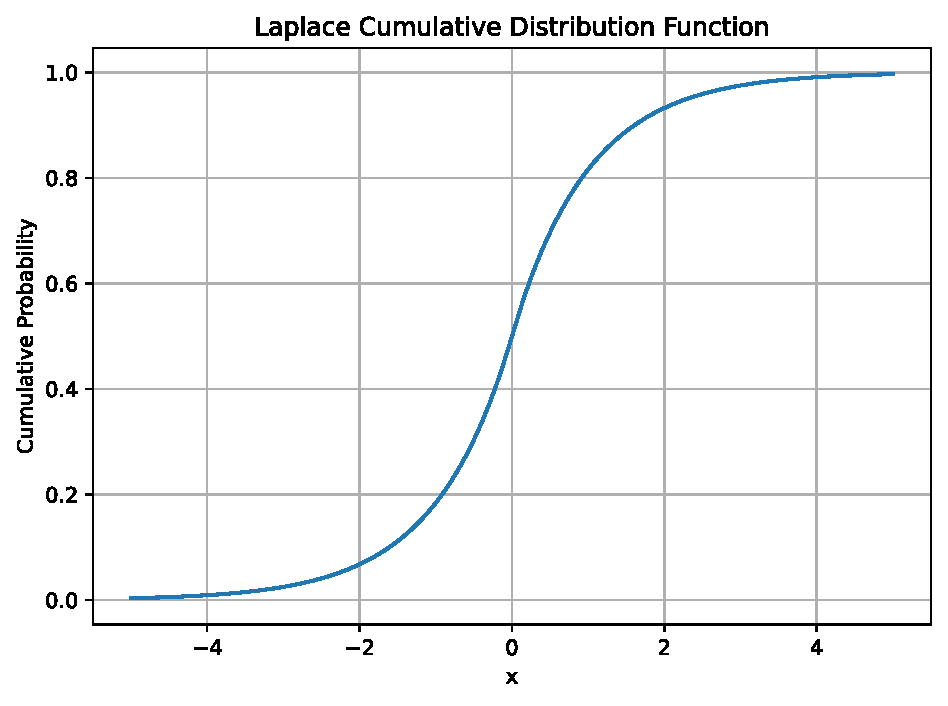
\includegraphics[width=1.0\linewidth]{Figures/laplace/laplace_cdf}
		\caption{Laplace Cumulative Density Function.}
		\label{fig:laplace distribution cdf}
		\end{figure}
	
		where $sgn(\cdot)$ denotes the sign function, while $F(x)$ represents the probability of a sample lying within the range $(-\infty, x]$. The cumulative distribution function (CDF) curve is illustrated in Fig.~\ref{fig:laplace distribution cdf}.
		
		In this work, we use the idea of maximum likelihood function. As above said, we can calculate the probability of the variable locating in the range $[x-\delta, x+\delta]$ by $F(x+\delta)-F(x-\delta)$. And we define the likelihood function as Eq~\eqref{eq:likelihood function}. 
		\begin{equation}
			L(x) = \sum_{1}^{49} F(x+\delta)-F(x-\delta)
			\label{eq:likelihood function}
		\end{equation}
	
		
		
		We aim to find the optimal depth value that maximizes the likelihood of observing the predictions within a narrow range centered around it. We said we use the idea of maximum likelihood function but not direct this method, because Maximum Likelihood Function is that we know about which distribution the real data follows, and we use the observed data to predict the distribution parameters. However, in our method, we use the predicted distribution to determine the observed position with maximum likelihood. We think our method is more like a multi-model fusion method. In Fig.~\ref{}, we give some examples of the application of our method.
		
		
	
	
	
	\section{Experiments}\label{sec:exp}
	\subsection{Dataset}
	\subsubsection{KITTI Dataset}
	The KITTI dataset is widely acknowledged as a standard benchmark in the field of 3D object detection. It comprises 7,481 images paired with finely calibrated 3D bounding boxes for training, as well as 7,518 samples designated for testing. We split the training set into two subsets: a training with 3,712 samples and a validation set with 3,769 samples. This division was employed for fine-tuning and optimizing hyperparameters during model development. For the final submissions to the KITTI test server, we adopted an approach inspired by PV-RCNN. In this instance, 80\% of the training samples were allocated for model training, while the remaining 20\% were set aside for validation.
	
	\subsubsection{Waymo Dataset}
	We perform experiments on Waymo dataset [47], which is a large-scale modern dataset for self-driving. It contains 798 sequences for training and 202 sequences for validation. We sample every $3^{rd}$ frame from the training sequence to form a small training set like CaDDN. The processed training sets have approximately 50k frames.
	
	\subsection{Implementation Details}
	In MSGA module, we use 1*1 convolution and leaky ReLU and 1*1 convolution along with a Sigmoid function to get the attention map. For enlarged RoI, we add no pixels, 10 pixels and 20 pixels, to each side of the RoI. We have test different configuration in the Sec~\ref{sec:exp}. We set $\sigma=0.1$ to refine our post processing process. The value of $\sigma$ is choosen based on the experiments. We use Adam as our optimizer, and set weight decay as 0.00001. We train our model for 200 epochs. At the first 5 epochs, we use the cosine function to transform the learning rate from 0.00001 to 0.001. The learning rate is set to 0.001 in the remaining epochs. And will decay 0.1 at the 90 and 120 epoch. In the training phase, we remove the frame with no ground truth label for more stable and robust training. 
	
	For data augmentation, we use random flip and random crop. After flipping and cropping, affine transformation will be applied on the cropped image to resize the image to the size of $(1280, 384)$ for batch processing. It should be noted that, after cropping and affine transformation, it may cause the processed image having black edge or remove some objects outside the picture, as depicted in Fig.~\ref{fig:affine trans}. For the first condition, for the keypoint of centerpoint that locates in the black space, we calculate their heatmap. For that outside the whole image, we do not calculate their heatmap. But in training phase, the heatmap of black edge do not participate into the loss calculation. For the second condition, if centers of all objects are outside the image, we random sample another item in the dataset.
\begin{table}[]
	\centering
	\caption{{Car results on KITTI Testing Dataset}}
	\label{tab:kitti_test}
	\resizebox{\columnwidth}{!}{%
		\begin{tabular}{ccccc}
			\toprule%第一道横线
			\multirow{2}{*}{{Method}} & \multicolumn{3}{c}{{Car(IoU=0.7)}}                & \multirow{2}{*}{{3D mAP}} \\ \cline{2-4}
			& {Easy}           & {Mod.}           & {Hard}           &                         \\ 
			\midrule%第二道横线
			{CLOCs\_SecCas~\cite{pang2020clocs}}           & {86.38}          & {78.45}          & {72.45}          & {79.09}                   \\
			{CLOCs\_SecRes*~\cite{pang2020clocs}}          & {85.35}          & {77.62}          & {72.96}          & {78.64}                   \\
			{CLOCs\_PVCas~\cite{pang2020clocs}}            & {88.94}          & {80.67}          & {77.15}          & {82.25}                   \\
			{Fast-CLOCs-PV~\cite{pang2022fast}}           & {89.11}          & {80.34}          & {76.98}          & {82.14}                   \\
			{C-CLOCs\_SecRes(ours)}         & {86.36}          & {78.42}          & {73.45}          & {79.41}                   \\
			{C-CLOCs\_VoxRes(ours)}         & {\textbf{90.12}} & {\textbf{81.56}} & {\textbf{78.23}} & {\textbf{83.30}}          \\ 
			\bottomrule%第三道横线
		\end{tabular}
	}
\end{table}

\begin{table}[]
	\centering
	\caption{{Car results on KITTI validation dataset}}
	\label{tab:kitti_valid}
	\resizebox{\columnwidth}{!}{%
		\begin{tabular}{ccccc}
			\toprule%第一道横线
			\multirow{2}{*}{{Method}} & \multicolumn{3}{c}{{Car(IoU=0.7)}}                & \multirow{2}{*}{{3D mAP}} \\ \cline{2-4}
			& {Easy}           & {Mod.}           & {Hard}           &                         \\ 
			\midrule%第二道横线
			{CLOCs\_SecCas~\cite{pang2020clocs}}           & {86.38}          & {78.45}          & {72.45}          & {79.09}                   \\
			{CLOCs\_SecRes*~\cite{pang2020clocs}}          & {85.35}          & {77.62}          & {72.96}          & {78.64}                   \\
			{CLOCs\_PVCas~\cite{pang2020clocs}}            & {88.94}          & {80.67}          & {77.15}          & {82.25}                   \\
			{Fast-CLOCs-PV~\cite{pang2022fast}}           & {89.11}          & {80.34}          & {76.98}          & {82.14}                   \\
			{C-CLOCs\_SecRes(ours)}         & {86.36}          & {78.42}          & {73.45}          & {79.41}                   \\
			{C-CLOCs\_VoxRes(ours)}         & {\textbf{90.12}} & {\textbf{81.56}} & {\textbf{78.23}} & {\textbf{83.30}}          \\ 
			\bottomrule%第三道横线
		\end{tabular}
	}
\end{table}


% Please add the following required packages to your document preamble:
% \usepackage{multirow}
% \usepackage{graphicx}
\begin{table}[]
	\centering
	\caption{Results of Waymo Validation Dataset}
	\label{tab:waymo_valid}
	\resizebox{\columnwidth}{!}{%
		\begin{tabular}{ccccc}
			\toprule%第一道横线
			\multirow{2}{*}{Methods} & \multicolumn{4}{c}{3D mAP/mAPH}       \\ \cline{2-5}
			& Overall & 0-30m & 30-50m & 50m-$\inf$ \\
			\midrule%第二道横线
			
			\multicolumn{5}{c}{Under Level 1(IoU=0.5)}                       \\
			\midrule%第二道横线
			
			PatchNet                 &         &       &        &            \\
			CaDDN                    &         &       &        &            \\
			PCT                      &         &       &        &            \\
			MonoJSG                  &         &       &        &            \\
			DID-M3D                  &         &       &        &            \\
			\midrule%第二道横线
			\multicolumn{5}{c}{Under Level 2(IoU=0.5)}                       \\
			\midrule%第二道横线
			PatchNet                 &         &       &        &            \\
			CaDDN                    &         &       &        &            \\
			PCT                      &         &       &        &            \\
			MonoJSG                  &         &       &        &            \\
			DID-M3D                  &         &       &        &        	 \\
			\bottomrule%第三道横线
		\end{tabular}%
	}
\end{table}
	\subsection{Experiment Results}
	\subsubsection{KITTI test dataset}
	We conduct experiments on the KITTI test dataset, and the comparison between our method and state-of-the-art approaches is presented in Table~\ref{tab:kitti_test}, where the best result are bolded. The results show that, our method outperforms other SOTA methods.
	
	\subsubsection{KITTI validation dataset} 
	We conduct experiments on the KITTI validation dataset, and the comparison between our method and other approaches is presented in Table~\ref{tab:kitti_valid}, where the best result are bolded. The results show that, our method outperforms other methods as well.
	
	\subsubsection{Waymo validation dataset} 
	We conduct experiments on the Waymo validation dataset, and the comparison between our method and other approaches is presented in Table~\ref{tab:waymo_valid}, where the best result are bolded. The results show that, our method outperforms other methods as well.
	\begin{figure*}[!t]
	\centering
	\includegraphics[width=1.0\linewidth]{Figures/qualitative_results/test.eps}
	\caption{Qualitative Results of KITTI test dataset.}
	\label{fig:qualitative result kitti test}
\end{figure*}
	\begin{figure*}[!t]
	\centering
	\includegraphics[width=1.0\linewidth]{Figures/qualitative_results/val.eps}
	\caption{Qualitative Results of KITTI validation dataset.}
	\label{fig:qualitative result kitti valid}
\end{figure*}
	\subsubsection{Qualitative results}
	The qualitative results are depicted in Fig~\ref{fig:qualitative result kitti test}.
	
	\subsubsection{title}
		\begin{table}[]
		\centering
		\caption{Effects of different components}
		\label{tab:diff_com}
		\resizebox{\columnwidth}{!}{%
			\begin{tabular}{cccccccc}
				\hline
				\multirow{2}{*}{{No.}}  & \multirow{2}{*}{MS}       & \multirow{2}{*}{GA}      & \multirow{2}{*}{PPP}       & \multicolumn{3}{c}{{Car (IoU=0.7)}} & \multirow{2}{*}{3D mAP} \\ \cline{5-7}
				& &                           &                           & Easy  & Mod.  & Hard  &       \\ \hline
				{(a)}& &                           &                           & 90.81 & 82.32 & 79.69 & 84.27 \\
				{(b)}& \checkmark   &              &                           & 91.38 & 82.76 & 79.90 & 84.68 \\
				{(c)}& & \checkmark &                           				& 90.51 & 82.04 & 81.25 & {84.60}  \\
				{(d)}& &                           & \checkmark 				& 91.13 & 82.53 & 79.85 & {84.50}  \\
				{(e)}& {\checkmark}  &{\checkmark}    & 			 				& {91.04} & {82.33} & {81.03} & {84.80}  \\
				{(f)}&           &{\checkmark}    & {\checkmark} 				& {90.86} & {82.19} & {81.25} & {84.77}  \\
				{(g)}&{\checkmark}   &              & {\checkmark} 				& {91.46} & {82.89} & {79.86} & {84.74}  \\
				{(h)}&\checkmark   & \checkmark   & \checkmark                & 91.26 & 82.61 & 81.17 & 85.01 \\ \hline
			\end{tabular}%
		}
	\end{table}

	\begin{table}[]
	\centering
	\caption{Effects of Multi-Scale Methods}
	\label{tab:multi_scale}
	\resizebox{\columnwidth}{!}{%
		\begin{tabular}{cccccccc}
			\hline
			\multirow{2}{*}{{No.}}  & \multirow{2}{*}{MS}       & \multirow{2}{*}{GA}      & \multirow{2}{*}{PPP}       & \multicolumn{3}{c}{{Car (IoU=0.7)}} & \multirow{2}{*}{3D mAP} \\ \cline{5-7}
			& &                           &                           & Easy  & Mod.  & Hard  &       \\ \hline
			{(a)}& &                           &                           & 90.81 & 82.32 & 79.69 & 84.27 \\
			{(b)}& \checkmark   &              &                           & 91.38 & 82.76 & 79.90 & 84.68 \\
			{(c)}& & \checkmark &                           				& 90.51 & 82.04 & 81.25 & {84.60}  \\
			{(d)}& &                           & \checkmark 				& 91.13 & 82.53 & 79.85 & {84.50}  \\
			{(e)}& {\checkmark}  &{\checkmark}    & 			 				& {91.04} & {82.33} & {81.03} & {84.80}  \\
			{(f)}&           &{\checkmark}    & {\checkmark} 				& {90.86} & {82.19} & {81.25} & {84.77}  \\
			{(g)}&{\checkmark}   &              & {\checkmark} 				& {91.46} & {82.89} & {79.86} & {84.74}  \\
			{(h)}&\checkmark   & \checkmark   & \checkmark                & 91.26 & 82.61 & 81.17 & 85.01 \\ \hline
		\end{tabular}%
	}
\end{table}

\begin{table}[]
	\centering
	\caption{Effects of Grid Attention Activation Function}
	\label{tab:grid attention activate function}
	\resizebox{\columnwidth}{!}{%
		\begin{tabular}{cccccccc}
			\hline
			\multirow{2}{*}{{No.}}  & \multirow{2}{*}{MS}       & \multirow{2}{*}{GA}      & \multirow{2}{*}{PPP}       & \multicolumn{3}{c}{{Car (IoU=0.7)}} & \multirow{2}{*}{3D mAP} \\ \cline{5-7}
			& &                           &                           & Easy  & Mod.  & Hard  &       \\ \hline
			{(a)}& &                           &                           & 90.81 & 82.32 & 79.69 & 84.27 \\
			{(b)}& \checkmark   &              &                           & 91.38 & 82.76 & 79.90 & 84.68 \\
			{(c)}& & \checkmark &                           				& 90.51 & 82.04 & 81.25 & {84.60}  \\
			{(d)}& &                           & \checkmark 				& 91.13 & 82.53 & 79.85 & {84.50}  \\
			{(e)}& {\checkmark}  &{\checkmark}    & 			 				& {91.04} & {82.33} & {81.03} & {84.80}  \\
			{(f)}&           &{\checkmark}    & {\checkmark} 				& {90.86} & {82.19} & {81.25} & {84.77}  \\
			{(g)}&{\checkmark}   &              & {\checkmark} 				& {91.46} & {82.89} & {79.86} & {84.74}  \\
			{(h)}&\checkmark   & \checkmark   & \checkmark                & 91.26 & 82.61 & 81.17 & 85.01 \\ \hline
		\end{tabular}%
	}
\end{table}

\begin{table}[]
	\centering
	\caption{Effects of Probabilistic Post Processing}
	\label{tab:ppp module}
	\resizebox{\columnwidth}{!}{%
		\begin{tabular}{cccccccc}
			\hline
			\multirow{2}{*}{{No.}}  & \multirow{2}{*}{MS}       & \multirow{2}{*}{GA}      & \multirow{2}{*}{PPP}       & \multicolumn{3}{c}{{Car (IoU=0.7)}} & \multirow{2}{*}{3D mAP} \\ \cline{5-7}
			& &                           &                           & Easy  & Mod.  & Hard  &       \\ \hline
			{(a)}& &                           &                           & 90.81 & 82.32 & 79.69 & 84.27 \\
			{(b)}& \checkmark   &              &                           & 91.38 & 82.76 & 79.90 & 84.68 \\
			{(c)}& & \checkmark &                           				& 90.51 & 82.04 & 81.25 & {84.60}  \\
			{(d)}& &                           & \checkmark 				& 91.13 & 82.53 & 79.85 & {84.50}  \\
			{(e)}& {\checkmark}  &{\checkmark}    & 			 				& {91.04} & {82.33} & {81.03} & {84.80}  \\
			{(f)}&           &{\checkmark}    & {\checkmark} 				& {90.86} & {82.19} & {81.25} & {84.77}  \\
			{(g)}&{\checkmark}   &              & {\checkmark} 				& {91.46} & {82.89} & {79.86} & {84.74}  \\
			{(h)}&\checkmark   & \checkmark   & \checkmark                & 91.26 & 82.61 & 81.17 & 85.01 \\ \hline
		\end{tabular}%
	}
\end{table}
	
	\subsection{Ablation Studies}
	\subsubsection{Influence of different components}
	We have tested the MSGA and PPP module in the Table~\ref{tab:diff_com}. We define our model that removes the MSGA and PPP module as the baseline.
	
	
	\subsubsection{Influence of Multi-Scale Methods}
	We have tested the enlarged pixels of RoI. For simplicity, we enlarged the with and the height with the same pixels. Moreover, we also enlarge the RoI proportionably. The results show that, if we enlarge the RoI proportionably, the performance will drop a lot, which may be caused by the scale-variant property of image.
	
	\subsubsection{Influence of Grid Attention Activation Function}
	To map the output of attention map to the range of $[0, 1]$, we select several functions for comparison, which is illustrated in Table~\ref{tab:grid attention activate function}. 
	
	\subsubsection{Influence of Probabilistic Posting Processing}
	We choose the $\delta$ in Probabilistic Posting Processing module to find the optimal hyper-parameters. If $\delta$ is set too small, the result will only concentrate on the prediction with lowest uncertainty. If $\delta$ is set too large, the difference will not obvious enough at different positions.

	

	
	

	%\bibliographystyle{IEEEtran}
	%\bibliography{references.bib}
	\begin{thebibliography}{1}
		\bibliographystyle{IEEEtran}	
		\bibitem{geometry3d}
		A. Mousavian, D. Anguelov, J. Flynn and J. Kosecka, “3D Bounding Box Estimation Using Deep Learning and Geometry,” in \textit{Proc. IEEE Conf. Comput. Vis. Pattern Recognit.}, Honolulu, HI, USA, 2017, pp. 7074-7082.
		
		\bibitem{roi10d}
		F. Manhardt, W. Kehl and A. Gaidon, “ROI-10D: Monocular Lifting of 2D Detection to 6D Pose and Metric Shape,” in \textit{Proc. IEEE/CVF Conf. Comput. Vis. Pattern Recognit.}, Long Beach, CA, USA. 2019, pp. 2069-2078.
		
		\bibitem{monopair}
		Y. Chen, L. Tai, K. Sun and M. Li, “MonoPair: Monocular 3D Object Detection Using Pairwise Spatial Relationships,” in \textit{Proc. IEEE/CVF Conf. Comput. Vis. Pattern Recognit.}, Seattle, WA, USA, 2020, pp. 12093-12102.
		
		\bibitem{smoke}
		Z. Liu, Z. Wu and R. Tóth, “Smoke: Single-stage monocular 3d object detection via keypoint estimation,” in \textit{Proc. IEEE Conf. Comput. Vis. Pattern Recognit.}, Seattle, WA, USA, 2020, pp. 996-997.
		
		\bibitem{polygon}
		Y. Cai, B. Li, Z. Jiao, H. Li, X. Zeng and X. Wang, “Monocular 3d object detection with decoupled structured polygon estimation and height-guided depth estimation,” in \textit{Proc. AAAI Conf. Artif. Intell.}, New York, New York, USA, 2020, pp. 10478-10485.
		
		\bibitem{monoflex}
		Y. Zhang, J. Lu and J. Zhou, “Objects are Different: Flexible Monocular 3D Object Detection,” in \textit{Proc. IEEE/CVF Conf. Comput. Vis. Pattern Recognit.}, Nashville, TN, USA, 2021, pp. 3289-3298.
		
		\bibitem{caddn}
		C. Reading, A. Harakeh, J. Chae and S. Waslander, “Categorical Depth Distribution Network for Monocular 3D Object Detection,” in \textit{Proc. IEEE/CVF Conf. Comput. Vis. Pattern Recognit.}, Nashville, TN, USA, 2021, pp. 8555-8564.
		
		\bibitem{gupnet}
		Y. Lu et al., “Geometry Uncertainty Projection Network for Monocular 3D Object Detection,” in \textit{Proc. IEEE/CVF Int. Conf. Comput. Vis.}, Montreal, Canada. 2021, pp. 3111-3121.
		
		\bibitem{dd3d}
		D. Park, R. Ambrus, V. Guizilini, J. Li and A. Gaidon, “Is Pseudo-Lidar needed for Monocular 3D Object detection?,” in \textit{Proc. IEEE/CVF Int. Conf. Comput. Vis.}, Montreal, Canada. 2021, pp. 3142-3152.
		
		\bibitem{monodde}
		Z. Li, Z. Qu, Y. Zhou, J. Liu, H. Wang and L. Jiang, “Diversity Matters: Fully Exploiting Depth Clues for Reliable Monocular 3D Object Detection,” in \textit{Proc. IEEE/CVF Conf. Comput. Vis. Pattern Recognit.}, New Orleans, LA, USA, 2022, pp. 2791-2800.
		
		\bibitem{didm3d}
		L. Peng, X. Wu, Z. Yang, H. Liu and D. Cai, “DID-M3D: Decoupling Instance Depth for Monocular 3D Object Detection,” in \textit{Eur. Conf. Comput. Vis.}, Tel-Aviv, Israel, 2022, pp. 71–88.
				
		\bibitem{imvoxelnet}
		D. Rukhovich, A. Vorontsova and A. Konushin, “ImVoxelNet: Image to Voxels Projection for Monocular and Multi-View General-Purpose 3D Object Detection,” in \textit{Proc. IEEE/CVF Winter Conf. Appl. Comput. Vis.}, Waikoloa, HI, USA. 2022, pp. 2397-2406.
		
		\bibitem{pgd}
		T. Wang, Z. Xinge, J. Pang and D. Lin, “Probabilistic and Geometric Depth: Detecting Objects in Perspective,” in \textit{Conf. on Robot. Learn.}, London, UK, 2022, pp. 1475-1485.
			
		\bibitem{monodtr}
		K. Huang, T. Wu, H. Su and W. Hsu, “MonoDTR: Monocular 3D Object Detection With Depth-Aware Transformer,” in \textit{Proc. IEEE/CVF Conf. Comput. Vis. Pattern Recognit.}, New Orleans, LA, USA, 2022,  pp. 4012-4021.
		
		
		\bibitem{monocon}
		X. Liu, N. Xue and T. Wu, “Learning Auxiliary Monocular Contexts Helps Monocular 3D Object Detection,” in \textit{Proc. AAAI Conf. Artif. Intell.}, Virtual, 2022, pp. 1810-1818.
		
		\bibitem{cie}
		Q. Ye, L. Jiang, W. Zhen and Y. Du, “Consistency of Implicit and Explicit Features Matters for Monocular 3D Object Detection,” 2022, \textit{arXiv:2207.07933}.
		
		\bibitem{monoxiver}
		X. Liu, C. Zheng, K. Cheng, N. Xue, G. Qi and T. Wu, “Monocular 3D Object Detection with Bounding Box Denoising in 3D by Perceiver,” in \textit{Proc. IEEE/CVF Int. Conf. Comput. Vis.}, Paris, 
		France. 2023, pp. 6436-6446.
		
		\bibitem{neurocs}
		Z. Min, B. Zhuang, S. Schulter, B. Liu, E. Dunn and M. Chandraker, “NeurOCS: Neural NOCS Supervision for Monocular 3D Object Localization,” in \textit{Proc. IEEE/CVF Conf. Comput. Vis. Pattern Recognit.}, Vancouver, Canada. 2023, pp. 21404-21414. 
		
		\bibitem{mononerd}
		J. Xu et al., “MonoNeRD: NeRF-like Representations for Monocular 3D Object Detection,” in \textit{Proc. IEEE/CVF Int. Conf. Comput. Vis.}, Paris, France. 2023, pp. 6814-6824. 
		
		\bibitem{monopgc}
		Z. Wu, Y. Gan, L. Wang, G. Chen and J. Pu, “MonoPGC: Monocular 3D Object Detection with Pixel Geometry Contexts,” in \textit{Int. Conf. Robot. Automat.}, London, UK. 2023, pp. 4842-4849. 
		
		\bibitem{gupnet++}
		Y.Lu et al., “GUPNet++: Geometry Uncertainty Propagation Network for Monocular 3D Object Detection.,” in \textit{Int. Conf. Robot. Automat.}, 2023, \textit{arXiv:2310.15624}.
		
		\bibitem{ssd-monodetr}
		X. He et al., “SSD-MonoDETR: Supervised Scale-Aware Deformable Transformer for Monocular 3D Object Detection,” in \textit{IEEE Trans. Intell. Veh.}, vol. 9, no. 1, pp. 555-567, Ian. 2024, doi: 10.1109/TIV.2023.3311949.
		
		\bibitem{mask-rcnn}
		K. He, G. Gkioxari, P. Dollar and R. Girshick, “Mask R-CNN,” in \textit{Proc. IEEE/CVF Int. Conf. Comput. Vis.}, Venice, Italy. 2023, pp. 6814-6824.
		
		\bibitem{patchnet}
		X. Ma, S. Liu, Z. Xia, H. Zhang and X. Zeng, “Rethinking pseudo-lidar representation,” in \textit{Eur. Conf. Comput. Vis.}, Virtual, 2020, pp. 311–327.
		
		\bibitem{pct}
		L. Wang et al., “Progressive coordinate transforms for monocular 3d object detection,” in \textit{Adv. Neural Inf. Process. Syst.}, Vol. 34, pp. 13364--13377, 2021.
		
		\bibitem{monojsg}
		Q. Lian, P. Li and X. Chen, “Monojsg: Joint semantic and geometric cost volume for monocular 3d object detection,” in \textit{Proc. IEEE/CVF Conf. Comput. Vis. Pattern Recognit.}, New Orleans, LA, USA, 2022, pp. 1070-1079.
		
		\bibitem{fast-rcnn}
		R. Girshick, “Fast R-CNN,” in \textit{Proc. IEEE/CVF Int. Conf. Comput. Vis.}, Santiago, Chile. 2015, pp. 1440-1448.
		
		\bibitem{roi-warp}
		J. Dai, K. He and J. Sun, “Instance-Aware Semantic Segmentation via Multi-Task Network Cascades,” in \textit{Proc. IEEE/CVF Conf. Comput. Vis. Pattern Recognit.}, Las Vegas, NV, USA, 2016, pp. 3150-3158.
	
		\bibitem{kitti}
		A. Geiger, P. Lenz, and R. Urtasun, “Are we ready for autonomous driving? The kitti vision benchmark suite,” in \textit{Proc. IEEE Conf. Comput. Vis. Pattern Recognit.}, Providence, RI, 2012, pp. 3354–3361.
		
		\bibitem{m3d-rpn}
		G. Brazil and X. Liu, “M3D-RPN: Monocular 3D Region Proposal Network for Object Detection,” in \textit{Proc. IEEE/CVF Int. Conf. Comput. Vis.}, Seoul, Korea. 2019, pp. 9287-9296.
		
		\bibitem{d4lcn}
		M. Ding, et.al., “Learning Depth-Guided Convolutions for Monocular 3D Object Detection,” in \textit{Proc. IEEE Conf. Comput. Vis. Pattern Recognit.}, Seattle, WA, USA, 2020, pp. 1000-1001.
		
		\bibitem{oft}
		T. Roddick, A. Kendall and R. Cipolla, “Orthographic Feature Transform for Monocular 3D Object Detection,” 2018, \textit{arXiv:1811.08188}.
		
		\bibitem{color-embeded}
		X. Ma, Z. Wang, H. Li, P. Zhang, W. Ouyang and X, Fan, “Accurate Monocular 3D Object Detection via Color-Embedded 3D Reconstruction for Autonomous Driving,” in \textit{Proc. IEEE/CVF Int. Conf. Comput. Vis.}, Seoul, Korea. 2019, pp. 6851-6860.
		
		\bibitem{mono-plidar}
		X. Weng, K. Kitani, “Monocular 3D Object Detection with Pseudo-LiDAR Point Cloud,” in \textit{Proc. IEEE/CVF Int. Conf. Comput. Vis.}, Seoul, Korea. 2019, pp. 0-0. 
		
		\bibitem{rtm3d}
		P. Li, H. Zhao, P. Liu and F. Cao, “RTM3D: Real-time Monocular 3D Detection from Object Keypoints for Autonomous Driving,” in \textit{Eur. Conf. Comput. Vis.}, Virtual, 2020, pp. 644-660.
		
		\bibitem{nerf}
		B. Mildenhall, P. Srinivasan, M. Tancik, J. Barron, R. Ramamoorthi and R. Ng, “NeRF: representing scenes as neural radiance fields for view synthesis,” in \textit{Commun. ACM}, vol. 65, no. 1, pp. 99–106, 2021.
		
		\bibitem{monodle}
		X. Ma et.al., “Delving Into Localization Errors for Monocular 3D Object Detection,” in \textit{Proc. IEEE/CVF Conf. Comput. Vis. Pattern Recognit.}, Nashville, TN, USA, 2021, pp. 4721-4730.
		
		\bibitem{m3dssd}
		S. Luo, H. Dai, L. Shao and Y. Ding, “M3DSSD: Monocular 3D Single Stage Object Detector,” in \textit{Proc. IEEE/CVF Conf. Comput. Vis. Pattern Recognit.}, Nashville, TN, USA, 2021, pp. 6145-6154.
		
		\bibitem{ddmp-3d}
		L. Wang et.al., “Depth-Conditioned Dynamic Message Propagation for Monocular 3D Object Detection,” in \textit{Proc. IEEE/CVF Conf. Comput. Vis. Pattern Recognit.}, Nashville, TN, USA, 2021, pp. 454-463.
		
		\bibitem{dla}
		F. Yu, D. Wang, E. Shelhamer, T. Darrell, “Deep Layer Aggregation,” in \textit{Proc. IEEE/CVF Conf. Comput. Vis. Pattern Recognit.}, 	Salt Lake City, UT, USA, 2018, pp.  2403-2412.
		
		\bibitem{centernet}
		X. Zhou, D. Wang, P. Krähenbühl, “Objects as points,” 2019, \textit{arXiv:1904.07850}.
		
		\bibitem{pyramid-rcnn}
		J. Mao, M. Niu, H. Bai, X. Liang, H. Xu, C. Xu, “Pyramid R-CNN: Towards Better Performance and Adaptability for 3D Object Detection,” in \textit{Proc. IEEE/CVF Int. Conf. Comput. Vis.}, Montreal, Canada. 2021, pp. 2723-2732. 
		
		\bibitem{leaky-relu}
		A. Maas, A. Hannun, A. Ng, “Rectifier nonlinearities improve neural network acoustic models,” in \textit{Proc. ICML}, 	Atlanta, USA. 2013. 
		
		
		
	\end{thebibliography}

% Please add the following required packages to your document preamble:
% \usepackage{longtable}
% Note: It may be necessary to compile the document several times to get a multi-page table to line up properly

	
	\begin{IEEEbiography}[{\includegraphics[width=1in,height=1.25in,clip,keepaspectratio]{Figures/zty}}]{Tingyu Zhang}
		Tingyu Zhang received the B.Sc. degree in Mathematics and Statistics from the Nanjing University of Information Science and Technology, Nanjing, China,
		in 2019. He is currently pursuing the Ph.D. degree
		in computer science and technology with Jilin University,
		Changchun. His current research interests
		include intelligent vehicles, point cloud analysis and 3D object detection.\end{IEEEbiography}
	
	\begin{IEEEbiography}[{\includegraphics[width=1in,height=1.25in,clip,keepaspectratio]{Figures/lgz}}]{Zhigang Liang}
		Zhigang Liang graduated from Jilin University with a bachelor's degree in Engineering mechanics in 2019. He is currently pursuing a PhD in Computer Science and Technology at Jilin University in Changchun. His current research interests include self-driving car digital twin testing and intelligent transportation.\end{IEEEbiography}
	
	\begin{IEEEbiography}[{\includegraphics[width=1in,height=1.25in,clip,keepaspectratio]{Figures/yyz}}]{Yanzhao Yang}
		Yanzhao Yang received his master's degree from Jilin University in 2011, major in Computer Science and Technology. He is currently pursuing the Ph.D degree in computer science and Technology with Jilin University, Changchun. His current research interests include intelligent vehicles, Physical Model of ADAS sensor and machine learning.\end{IEEEbiography}
	
	\begin{IEEEbiography}[{\includegraphics[width=1in,height=1.25in,clip,keepaspectratio]{Figures/yxy}}]{Xinyu Yang}
		Xinyu Yang received her master's degree in computer technique from Jilin University of science and technology. Her research interests include vehicular networks and intelligent driving, especially for privacy protection. She currently works for China Automotive Innovation Corporation.\end{IEEEbiography}
	
	\begin{IEEEbiography}[{\includegraphics[width=1in,height=1.25in,clip,keepaspectratio]{Figures/zy}}]{Yu Zhu}
		Yu Zhu received the B.Sc. degree in computer
		science and technology from the Changchun University
		of Science and Technology, Changchun, China,
		in 2018. He is currently pursuing the Ph.D. degree
		in computer science and technology with Jilin University,
		Changchun. His current research interests
		include connected and autonomous vehicle testing,
		hardware-in-the-loop test solutions, and testing scenario
		library generation.\end{IEEEbiography}
	
	\begin{IEEEbiography}[{\includegraphics[width=1in,height=1.25in,clip,keepaspectratio]{Figures/wj}}]{Jian Wang}
		Jian Wang received the B.Sc., M.Sc., and Ph.D.
		degrees in computer science from Jilin University,
		Changchun, China, in 2004, 2007, and 2011, respectively.
		He is currently a Professor with the College of
		Computer Science and Technology, Jilin University.
		He has published over 60 articles in international
		journals. His research interests include wireless communication
		and vehicular networks, especially for
		network security and privacy protection.\end{IEEEbiography}






\end{document}


